% Options for packages loaded elsewhere
\PassOptionsToPackage{unicode}{hyperref}
\PassOptionsToPackage{hyphens}{url}
%
\documentclass[
]{article}
\usepackage{amsmath,amssymb}
\usepackage{lmodern}
\usepackage{iftex}
\ifPDFTeX
  \usepackage[T1]{fontenc}
  \usepackage[utf8]{inputenc}
  \usepackage{textcomp} % provide euro and other symbols
\else % if luatex or xetex
  \usepackage{unicode-math}
  \defaultfontfeatures{Scale=MatchLowercase}
  \defaultfontfeatures[\rmfamily]{Ligatures=TeX,Scale=1}
\fi
% Use upquote if available, for straight quotes in verbatim environments
\IfFileExists{upquote.sty}{\usepackage{upquote}}{}
\IfFileExists{microtype.sty}{% use microtype if available
  \usepackage[]{microtype}
  \UseMicrotypeSet[protrusion]{basicmath} % disable protrusion for tt fonts
}{}
\makeatletter
\@ifundefined{KOMAClassName}{% if non-KOMA class
  \IfFileExists{parskip.sty}{%
    \usepackage{parskip}
  }{% else
    \setlength{\parindent}{0pt}
    \setlength{\parskip}{6pt plus 2pt minus 1pt}}
}{% if KOMA class
  \KOMAoptions{parskip=half}}
\makeatother
\usepackage{xcolor}
\usepackage[margin=1in]{geometry}
\usepackage{color}
\usepackage{fancyvrb}
\newcommand{\VerbBar}{|}
\newcommand{\VERB}{\Verb[commandchars=\\\{\}]}
\DefineVerbatimEnvironment{Highlighting}{Verbatim}{commandchars=\\\{\}}
% Add ',fontsize=\small' for more characters per line
\usepackage{framed}
\definecolor{shadecolor}{RGB}{248,248,248}
\newenvironment{Shaded}{\begin{snugshade}}{\end{snugshade}}
\newcommand{\AlertTok}[1]{\textcolor[rgb]{0.94,0.16,0.16}{#1}}
\newcommand{\AnnotationTok}[1]{\textcolor[rgb]{0.56,0.35,0.01}{\textbf{\textit{#1}}}}
\newcommand{\AttributeTok}[1]{\textcolor[rgb]{0.77,0.63,0.00}{#1}}
\newcommand{\BaseNTok}[1]{\textcolor[rgb]{0.00,0.00,0.81}{#1}}
\newcommand{\BuiltInTok}[1]{#1}
\newcommand{\CharTok}[1]{\textcolor[rgb]{0.31,0.60,0.02}{#1}}
\newcommand{\CommentTok}[1]{\textcolor[rgb]{0.56,0.35,0.01}{\textit{#1}}}
\newcommand{\CommentVarTok}[1]{\textcolor[rgb]{0.56,0.35,0.01}{\textbf{\textit{#1}}}}
\newcommand{\ConstantTok}[1]{\textcolor[rgb]{0.00,0.00,0.00}{#1}}
\newcommand{\ControlFlowTok}[1]{\textcolor[rgb]{0.13,0.29,0.53}{\textbf{#1}}}
\newcommand{\DataTypeTok}[1]{\textcolor[rgb]{0.13,0.29,0.53}{#1}}
\newcommand{\DecValTok}[1]{\textcolor[rgb]{0.00,0.00,0.81}{#1}}
\newcommand{\DocumentationTok}[1]{\textcolor[rgb]{0.56,0.35,0.01}{\textbf{\textit{#1}}}}
\newcommand{\ErrorTok}[1]{\textcolor[rgb]{0.64,0.00,0.00}{\textbf{#1}}}
\newcommand{\ExtensionTok}[1]{#1}
\newcommand{\FloatTok}[1]{\textcolor[rgb]{0.00,0.00,0.81}{#1}}
\newcommand{\FunctionTok}[1]{\textcolor[rgb]{0.00,0.00,0.00}{#1}}
\newcommand{\ImportTok}[1]{#1}
\newcommand{\InformationTok}[1]{\textcolor[rgb]{0.56,0.35,0.01}{\textbf{\textit{#1}}}}
\newcommand{\KeywordTok}[1]{\textcolor[rgb]{0.13,0.29,0.53}{\textbf{#1}}}
\newcommand{\NormalTok}[1]{#1}
\newcommand{\OperatorTok}[1]{\textcolor[rgb]{0.81,0.36,0.00}{\textbf{#1}}}
\newcommand{\OtherTok}[1]{\textcolor[rgb]{0.56,0.35,0.01}{#1}}
\newcommand{\PreprocessorTok}[1]{\textcolor[rgb]{0.56,0.35,0.01}{\textit{#1}}}
\newcommand{\RegionMarkerTok}[1]{#1}
\newcommand{\SpecialCharTok}[1]{\textcolor[rgb]{0.00,0.00,0.00}{#1}}
\newcommand{\SpecialStringTok}[1]{\textcolor[rgb]{0.31,0.60,0.02}{#1}}
\newcommand{\StringTok}[1]{\textcolor[rgb]{0.31,0.60,0.02}{#1}}
\newcommand{\VariableTok}[1]{\textcolor[rgb]{0.00,0.00,0.00}{#1}}
\newcommand{\VerbatimStringTok}[1]{\textcolor[rgb]{0.31,0.60,0.02}{#1}}
\newcommand{\WarningTok}[1]{\textcolor[rgb]{0.56,0.35,0.01}{\textbf{\textit{#1}}}}
\usepackage{graphicx}
\makeatletter
\def\maxwidth{\ifdim\Gin@nat@width>\linewidth\linewidth\else\Gin@nat@width\fi}
\def\maxheight{\ifdim\Gin@nat@height>\textheight\textheight\else\Gin@nat@height\fi}
\makeatother
% Scale images if necessary, so that they will not overflow the page
% margins by default, and it is still possible to overwrite the defaults
% using explicit options in \includegraphics[width, height, ...]{}
\setkeys{Gin}{width=\maxwidth,height=\maxheight,keepaspectratio}
% Set default figure placement to htbp
\makeatletter
\def\fps@figure{htbp}
\makeatother
\setlength{\emergencystretch}{3em} % prevent overfull lines
\providecommand{\tightlist}{%
  \setlength{\itemsep}{0pt}\setlength{\parskip}{0pt}}
\setcounter{secnumdepth}{-\maxdimen} % remove section numbering
\ifLuaTeX
  \usepackage{selnolig}  % disable illegal ligatures
\fi
\IfFileExists{bookmark.sty}{\usepackage{bookmark}}{\usepackage{hyperref}}
\IfFileExists{xurl.sty}{\usepackage{xurl}}{} % add URL line breaks if available
\urlstyle{same} % disable monospaced font for URLs
\hypersetup{
  pdftitle={Homework 6},
  pdfauthor={PSTAT 131/231},
  hidelinks,
  pdfcreator={LaTeX via pandoc}}

\title{Homework 6}
\author{PSTAT 131/231}
\date{}

\begin{document}
\maketitle

{
\setcounter{tocdepth}{2}
\tableofcontents
}
\hypertarget{tree-based-models}{%
\subsection{Tree-Based Models}\label{tree-based-models}}

For this assignment, we will continue working with the file
\texttt{"pokemon.csv"}, found in \texttt{/data}. The file is from
Kaggle: \url{https://www.kaggle.com/abcsds/pokemon}.

The \href{https://www.pokemon.com/us/}{Pokémon} franchise encompasses
video games, TV shows, movies, books, and a card game. This data set was
drawn from the video game series and contains statistics about 721
Pokémon, or ``pocket monsters.'' In Pokémon games, the user plays as a
trainer who collects, trades, and battles Pokémon to (a) collect all the
Pokémon and (b) become the champion Pokémon trainer.

Each Pokémon has a
\href{https://bulbapedia.bulbagarden.net/wiki/Type}{primary type} (some
even have secondary types). Based on their type, a Pokémon is strong
against some types, and vulnerable to others. (Think rock, paper,
scissors.) A Fire-type Pokémon, for example, is vulnerable to Water-type
Pokémon, but strong against Grass-type.

\begin{figure}
\centering
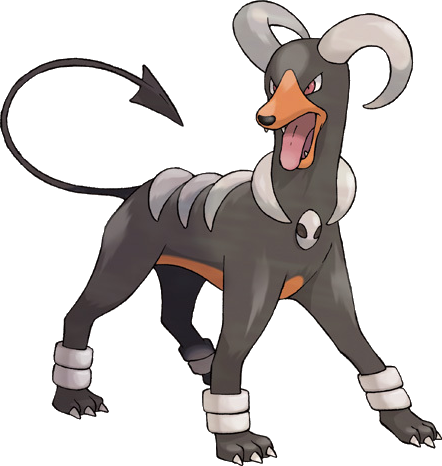
\includegraphics[width=2.08333in,height=\textheight]{images/houndoom.jpg}
\caption{Fig 1. Houndoom, a Dark/Fire-type canine Pokémon from
Generation II.}
\end{figure}

\begin{Shaded}
\begin{Highlighting}[]
\FunctionTok{library}\NormalTok{(ggplot2)}
\FunctionTok{library}\NormalTok{(dplyr)}
\FunctionTok{library}\NormalTok{(tidyverse)}
\FunctionTok{library}\NormalTok{(tidymodels)}
\FunctionTok{library}\NormalTok{(corrplot)}
\FunctionTok{library}\NormalTok{(rpart.plot)}
\FunctionTok{library}\NormalTok{(randomForest)}
\FunctionTok{library}\NormalTok{(ranger)}
\FunctionTok{library}\NormalTok{(vip)}
\FunctionTok{library}\NormalTok{(xgboost)}
\FunctionTok{library}\NormalTok{(pROC)}
\FunctionTok{library}\NormalTok{(janitor)}
\end{Highlighting}
\end{Shaded}

The goal of this assignment is to build a statistical learning model
that can predict the \textbf{primary type} of a Pokémon based on its
generation, legendary status, and six battle statistics.

\textbf{Note: Fitting ensemble tree-based models can take a little while
to run. Consider running your models outside of the .Rmd, storing the
results, and loading them in your .Rmd to minimize time to knit.}

\hypertarget{exercise-1}{%
\subsubsection{Exercise 1}\label{exercise-1}}

Read in the data and set things up as in Homework 5:

\begin{itemize}
\tightlist
\item
  Use \texttt{clean\_names()}
\item
  Filter out the rarer Pokémon types
\item
  Convert \texttt{type\_1} and \texttt{legendary} to factors
\end{itemize}

\begin{Shaded}
\begin{Highlighting}[]
\FunctionTok{library}\NormalTok{(janitor)}

\NormalTok{Pokemon }\OtherTok{\textless{}{-}} \FunctionTok{read\_csv}\NormalTok{(}\StringTok{"D:/UCSB/Spring\_2022/PSTAT 131/PSTAT\_131\_HW/HW2/PSTAT{-}131/homework{-}6/data/Pokemon.csv"}\NormalTok{)}
\NormalTok{Pokemon }\OtherTok{=} \FunctionTok{clean\_names}\NormalTok{(Pokemon)}
\end{Highlighting}
\end{Shaded}

\begin{Shaded}
\begin{Highlighting}[]
\NormalTok{Pokemon\_ra }\OtherTok{=}\NormalTok{ Pokemon }\SpecialCharTok{\%\textgreater{}\%} \FunctionTok{filter}\NormalTok{(type\_1 }\SpecialCharTok{==} \StringTok{"Bug"} \SpecialCharTok{|}\NormalTok{ type\_1 }\SpecialCharTok{==} \StringTok{"Fire"} \SpecialCharTok{|} 
\NormalTok{                                type\_1 }\SpecialCharTok{==} \StringTok{"Grass"} \SpecialCharTok{|}\NormalTok{ type\_1 }\SpecialCharTok{==} \StringTok{"Grass"} \SpecialCharTok{|}
\NormalTok{                                type\_1 }\SpecialCharTok{==} \StringTok{"Normal"} \SpecialCharTok{|}\NormalTok{ type\_1 }\SpecialCharTok{==} \StringTok{"Water"} \SpecialCharTok{|}
\NormalTok{                                type\_1 }\SpecialCharTok{==} \StringTok{"Psychic"}\NormalTok{)  }

\NormalTok{Pokemon\_ra }\OtherTok{=}\NormalTok{ Pokemon\_ra }\SpecialCharTok{\%\textgreater{}\%} 
  \FunctionTok{mutate}\NormalTok{(}\AttributeTok{legendary =} \FunctionTok{as.factor}\NormalTok{(legendary)) }\SpecialCharTok{\%\textgreater{}\%}
  \FunctionTok{mutate}\NormalTok{(}\AttributeTok{type\_1 =} \FunctionTok{as.factor}\NormalTok{(type\_1))}
\end{Highlighting}
\end{Shaded}

Do an initial split of the data; you can choose the percentage for
splitting. Stratify on the outcome variable.

\begin{Shaded}
\begin{Highlighting}[]
\FunctionTok{set.seed}\NormalTok{(}\DecValTok{3435}\NormalTok{)}
\NormalTok{Pokemon\_ra\_split }\OtherTok{=} \FunctionTok{initial\_split}\NormalTok{(Pokemon\_ra, }\AttributeTok{prop=}\FloatTok{0.85}\NormalTok{, }\AttributeTok{strata =}\NormalTok{ type\_1)}
\NormalTok{typeI\_train }\OtherTok{=} \FunctionTok{training}\NormalTok{(Pokemon\_ra\_split)}
\NormalTok{typeI\_test }\OtherTok{=} \FunctionTok{testing}\NormalTok{(Pokemon\_ra\_split)}
\end{Highlighting}
\end{Shaded}

Fold the training set using \emph{v}-fold cross-validation, with
\texttt{v\ =\ 5}. Stratify on the outcome variable.

\begin{Shaded}
\begin{Highlighting}[]
\FunctionTok{set.seed}\NormalTok{(}\DecValTok{3435}\NormalTok{)}
\NormalTok{typeI\_fold }\OtherTok{=} \FunctionTok{vfold\_cv}\NormalTok{(typeI\_train, }\AttributeTok{v=}\DecValTok{5}\NormalTok{, }\AttributeTok{strata =}\NormalTok{ type\_1)}
\end{Highlighting}
\end{Shaded}

Set up a recipe to predict \texttt{type\_1} with \texttt{legendary},
\texttt{generation}, \texttt{sp\_atk}, \texttt{attack}, \texttt{speed},
\texttt{defense}, \texttt{hp}, and \texttt{sp\_def}:

\begin{itemize}
\tightlist
\item
  Dummy-code \texttt{legendary} and \texttt{generation};
\item
  Center and scale all predictors.
\end{itemize}

\begin{Shaded}
\begin{Highlighting}[]
\NormalTok{typeI\_recipe }\OtherTok{=} \FunctionTok{recipe}\NormalTok{(type\_1 }\SpecialCharTok{\textasciitilde{}}\NormalTok{ legendary }\SpecialCharTok{+}\NormalTok{ generation }\SpecialCharTok{+}\NormalTok{ sp\_atk }\SpecialCharTok{+} 
\NormalTok{                      attack }\SpecialCharTok{+}\NormalTok{  speed }\SpecialCharTok{+}\NormalTok{ defense }\SpecialCharTok{+}\NormalTok{ hp }\SpecialCharTok{+}\NormalTok{ sp\_def,}
                      \AttributeTok{data =}\NormalTok{ typeI\_train) }\SpecialCharTok{\%\textgreater{}\%}
  \FunctionTok{step\_dummy}\NormalTok{(}\FunctionTok{all\_nominal\_predictors}\NormalTok{()) }\SpecialCharTok{\%\textgreater{}\%} 
  \FunctionTok{step\_normalize}\NormalTok{(}\FunctionTok{all\_predictors}\NormalTok{())}
\end{Highlighting}
\end{Shaded}

\begin{Shaded}
\begin{Highlighting}[]
\FunctionTok{head}\NormalTok{(Pokemon\_ra)}
\end{Highlighting}
\end{Shaded}

\begin{verbatim}
## # A tibble: 6 x 13
##   number name       type_1 type_2 total    hp attack defense sp_atk sp_def speed
##    <dbl> <chr>      <fct>  <chr>  <dbl> <dbl>  <dbl>   <dbl>  <dbl>  <dbl> <dbl>
## 1      1 Bulbasaur  Grass  Poison   318    45     49      49     65     65    45
## 2      2 Ivysaur    Grass  Poison   405    60     62      63     80     80    60
## 3      3 Venusaur   Grass  Poison   525    80     82      83    100    100    80
## 4      3 VenusaurM~ Grass  Poison   625    80    100     123    122    120    80
## 5      4 Charmander Fire   <NA>     309    39     52      43     60     50    65
## 6      5 Charmeleon Fire   <NA>     405    58     64      58     80     65    80
## # ... with 2 more variables: generation <dbl>, legendary <fct>
\end{verbatim}

\hypertarget{exercise-2}{%
\subsubsection{Exercise 2}\label{exercise-2}}

Create a correlation matrix of the training set, using the
\texttt{corrplot} package. \emph{Note: You can choose how to handle the
continuous variables for this plot; justify your decision(s).}

What relationships, if any, do you notice? Do these relationships make
sense to you?

\begin{Shaded}
\begin{Highlighting}[]
\NormalTok{typeI\_train }\SpecialCharTok{\%\textgreater{}\%} \FunctionTok{select}\NormalTok{(total, hp, attack, defense, }
\NormalTok{                       sp\_atk, sp\_def, speed, generation) }\SpecialCharTok{\%\textgreater{}\%}
  \FunctionTok{cor}\NormalTok{() }\SpecialCharTok{\%\textgreater{}\%}
  \FunctionTok{corrplot}\NormalTok{(}\AttributeTok{method =} \StringTok{"square"}\NormalTok{, }\AttributeTok{type =} \StringTok{"lower"}\NormalTok{, }\AttributeTok{diag =}\NormalTok{ F)}
\end{Highlighting}
\end{Shaded}

\includegraphics{homework-6_files/figure-latex/unnamed-chunk-8-1.pdf}

\textbf{Solution: } I found \emph{total} is positively correlated with a
few variables, such as \emph{attack}, \emph{sp\_atk}, and
\emph{sp\_def}. This makes sense since the latter values contribute to
the value of the \emph{total}. In addition, \emph{defense} is positive
correlated with \emph{sp\_def}, which is also reasonable.

\hypertarget{exercise-3}{%
\subsubsection{Exercise 3}\label{exercise-3}}

First, set up a decision tree model and workflow. Tune the
\texttt{cost\_complexity} hyperparameter. Use the same levels we used in
Lab 7 -- that is, \texttt{range\ =\ c(-3,\ -1)}. Specify that the metric
we want to optimize is \texttt{roc\_auc}.

Print an \texttt{autoplot()} of the results. What do you observe? Does a
single decision tree perform better with a smaller or larger complexity
penalty?

\begin{Shaded}
\begin{Highlighting}[]
\CommentTok{\# general decision tree spec}
\NormalTok{tree\_spec }\OtherTok{\textless{}{-}} \FunctionTok{decision\_tree}\NormalTok{() }\SpecialCharTok{\%\textgreater{}\%}
  \FunctionTok{set\_engine}\NormalTok{(}\StringTok{"rpart"}\NormalTok{)}
\CommentTok{\# class decision tree engine }
\NormalTok{class\_tree\_spec }\OtherTok{\textless{}{-}}\NormalTok{ tree\_spec }\SpecialCharTok{\%\textgreater{}\%}
  \FunctionTok{set\_mode}\NormalTok{(}\StringTok{"classification"}\NormalTok{)}

\NormalTok{class\_tree\_wf }\OtherTok{\textless{}{-}} \FunctionTok{workflow}\NormalTok{() }\SpecialCharTok{\%\textgreater{}\%}
  \FunctionTok{add\_model}\NormalTok{(class\_tree\_spec }\SpecialCharTok{\%\textgreater{}\%} \FunctionTok{set\_args}\NormalTok{(}\AttributeTok{cost\_complexity =} \FunctionTok{tune}\NormalTok{())) }\SpecialCharTok{\%\textgreater{}\%}
  \FunctionTok{add\_recipe}\NormalTok{(typeI\_recipe)}
\end{Highlighting}
\end{Shaded}

\begin{Shaded}
\begin{Highlighting}[]
\FunctionTok{set.seed}\NormalTok{(}\DecValTok{3435}\NormalTok{)}
\NormalTok{param\_grid }\OtherTok{\textless{}{-}} \FunctionTok{grid\_regular}\NormalTok{(}\FunctionTok{cost\_complexity}\NormalTok{(}\AttributeTok{range =} \FunctionTok{c}\NormalTok{(}\SpecialCharTok{{-}}\DecValTok{3}\NormalTok{, }\SpecialCharTok{{-}}\DecValTok{1}\NormalTok{)), }\AttributeTok{levels =} \DecValTok{10}\NormalTok{)}

\NormalTok{tune\_res }\OtherTok{\textless{}{-}} \FunctionTok{tune\_grid}\NormalTok{(}
\NormalTok{  class\_tree\_wf, }
  \AttributeTok{resamples =}\NormalTok{ typeI\_fold, }
  \AttributeTok{grid =}\NormalTok{ param\_grid, }
  \AttributeTok{metrics =} \FunctionTok{metric\_set}\NormalTok{(roc\_auc)}
\NormalTok{)}
\end{Highlighting}
\end{Shaded}

\begin{Shaded}
\begin{Highlighting}[]
\FunctionTok{autoplot}\NormalTok{(tune\_res)}
\end{Highlighting}
\end{Shaded}

\includegraphics{homework-6_files/figure-latex/unnamed-chunk-11-1.pdf}

\hypertarget{exercise-4}{%
\subsubsection{Exercise 4}\label{exercise-4}}

What is the \texttt{roc\_auc} of your best-performing pruned decision
tree on the folds? \emph{Hint: Use \texttt{collect\_metrics()} and
\texttt{arrange()}.}

\begin{Shaded}
\begin{Highlighting}[]
\NormalTok{m1 }\OtherTok{=} \FunctionTok{collect\_metrics}\NormalTok{(tune\_res) }\SpecialCharTok{\%\textgreater{}\%} \FunctionTok{arrange}\NormalTok{(}\FunctionTok{desc}\NormalTok{(mean)) }\SpecialCharTok{\%\textgreater{}\%} \FunctionTok{head}\NormalTok{()}
\NormalTok{m1}
\end{Highlighting}
\end{Shaded}

\begin{verbatim}
## # A tibble: 6 x 7
##   cost_complexity .metric .estimator  mean     n std_err .config              
##             <dbl> <chr>   <chr>      <dbl> <int>   <dbl> <chr>                
## 1         0.001   roc_auc hand_till  0.649     5  0.0217 Preprocessor1_Model01
## 2         0.00167 roc_auc hand_till  0.649     5  0.0217 Preprocessor1_Model02
## 3         0.0129  roc_auc hand_till  0.647     5  0.0257 Preprocessor1_Model06
## 4         0.00278 roc_auc hand_till  0.647     5  0.0216 Preprocessor1_Model03
## 5         0.0215  roc_auc hand_till  0.645     5  0.0119 Preprocessor1_Model07
## 6         0.00464 roc_auc hand_till  0.644     5  0.0207 Preprocessor1_Model04
\end{verbatim}

\hypertarget{exercise-5}{%
\subsubsection{Exercise 5}\label{exercise-5}}

Using \texttt{rpart.plot}, fit and visualize your best-performing pruned
decision tree with the \emph{training} set.

\begin{Shaded}
\begin{Highlighting}[]
\NormalTok{best\_complexity }\OtherTok{=} \FunctionTok{select\_best}\NormalTok{(tune\_res)}

\NormalTok{class\_tree\_final }\OtherTok{\textless{}{-}} \FunctionTok{finalize\_workflow}\NormalTok{(class\_tree\_wf, best\_complexity)}

\NormalTok{class\_tree\_final\_fit }\OtherTok{\textless{}{-}} \FunctionTok{fit}\NormalTok{(class\_tree\_final, }\AttributeTok{data =}\NormalTok{ typeI\_train)}
\end{Highlighting}
\end{Shaded}

\begin{Shaded}
\begin{Highlighting}[]
\NormalTok{class\_tree\_final\_fit }\SpecialCharTok{\%\textgreater{}\%}
  \FunctionTok{extract\_fit\_engine}\NormalTok{() }\SpecialCharTok{\%\textgreater{}\%}
  \FunctionTok{rpart.plot}\NormalTok{()}
\end{Highlighting}
\end{Shaded}

\includegraphics{homework-6_files/figure-latex/unnamed-chunk-14-1.pdf}

\hypertarget{exercise-5-1}{%
\subsubsection{Exercise 5}\label{exercise-5-1}}

Now set up a random forest model and workflow. Use the \texttt{ranger}
engine and set \texttt{importance\ =\ "impurity"}. Tune \texttt{mtry},
\texttt{trees}, and \texttt{min\_n}. Using the documentation for
\texttt{rand\_forest()}, explain in your own words what each of these
hyperparameters represent.

Create a regular grid with 8 levels each. You can choose plausible
ranges for each hyperparameter. Note that \texttt{mtry} should not be
smaller than 1 or larger than 8. \textbf{Explain why not. What type of
model would \texttt{mtry\ =\ 8} represent?}

\begin{Shaded}
\begin{Highlighting}[]
\NormalTok{rf\_spec }\OtherTok{=} \FunctionTok{rand\_forest}\NormalTok{(}\AttributeTok{mtry =} \FunctionTok{tune}\NormalTok{(), }\AttributeTok{trees =} \FunctionTok{tune}\NormalTok{(), }\AttributeTok{min\_n =} \FunctionTok{tune}\NormalTok{()) }\SpecialCharTok{\%\textgreater{}\%}
  \FunctionTok{set\_engine}\NormalTok{(}\StringTok{"ranger"}\NormalTok{, }\AttributeTok{importance =} \StringTok{"impurity"}\NormalTok{) }\SpecialCharTok{\%\textgreater{}\%}
  \FunctionTok{set\_mode}\NormalTok{(}\StringTok{"classification"}\NormalTok{)}
\end{Highlighting}
\end{Shaded}

\begin{Shaded}
\begin{Highlighting}[]
\NormalTok{rf\_wkflw }\OtherTok{=} \FunctionTok{workflow}\NormalTok{() }\SpecialCharTok{\%\textgreater{}\%} 
  \FunctionTok{add\_recipe}\NormalTok{(typeI\_recipe) }\SpecialCharTok{\%\textgreater{}\%}
  \FunctionTok{add\_model}\NormalTok{(rf\_spec)}
\end{Highlighting}
\end{Shaded}

\begin{Shaded}
\begin{Highlighting}[]
\NormalTok{rf\_grid }\OtherTok{=} \FunctionTok{grid\_regular}\NormalTok{(}\FunctionTok{mtry}\NormalTok{(}\AttributeTok{range =} \FunctionTok{c}\NormalTok{(}\DecValTok{1}\NormalTok{,}\DecValTok{8}\NormalTok{)), }
                       \FunctionTok{trees}\NormalTok{(}\AttributeTok{range =} \FunctionTok{c}\NormalTok{(}\DecValTok{50}\NormalTok{,}\DecValTok{1000}\NormalTok{)),}
                       \FunctionTok{min\_n}\NormalTok{(}\AttributeTok{range =} \FunctionTok{c}\NormalTok{(}\DecValTok{2}\NormalTok{, }\DecValTok{40}\NormalTok{)),}
                       \AttributeTok{levels =} \DecValTok{8}\NormalTok{)}
\end{Highlighting}
\end{Shaded}

\begin{enumerate}
\def\labelenumi{\arabic{enumi}.}
\item
  mtry: the number of predictors that will be randomly sampled at each
  split when creating the trees models. It depends on our recipe which
  contains 8 predictors.
\item
  trees: number of trees contained in the ensemble.
\item
  min\_n: minimum number of data points in a node that are required for
  the node to be split further
\end{enumerate}

Above parameters are all integers. mtry = 8 represents that all
predictors from the recipe in the training set will be randomly sampled
to create a random forest model.

\hypertarget{exercise-6}{%
\subsubsection{Exercise 6}\label{exercise-6}}

Specify \texttt{roc\_auc} as a metric. Tune the model and print an
\texttt{autoplot()} of the results. What do you observe? What values of
the hyperparameters seem to yield the best performance?

\begin{Shaded}
\begin{Highlighting}[]
\FunctionTok{set.seed}\NormalTok{(}\DecValTok{3435}\NormalTok{)}
\CommentTok{\#rf\_tune\_res = tune\_grid(}
  \CommentTok{\#rf\_wkflw,}
  \CommentTok{\#resamples = typeI\_fold, }
  \CommentTok{\#grid = rf\_grid,}
  \CommentTok{\#metrics = metric\_set(roc\_auc)}
\CommentTok{\#)}
\end{Highlighting}
\end{Shaded}

\begin{Shaded}
\begin{Highlighting}[]
\FunctionTok{load}\NormalTok{(}\AttributeTok{file =} \StringTok{"rf.Rdata"}\NormalTok{)}
\end{Highlighting}
\end{Shaded}

\begin{Shaded}
\begin{Highlighting}[]
\FunctionTok{autoplot}\NormalTok{(rf\_tune\_res)}
\end{Highlighting}
\end{Shaded}

\includegraphics{homework-6_files/figure-latex/unnamed-chunk-20-1.pdf}

\hypertarget{exercise-7}{%
\subsubsection{Exercise 7}\label{exercise-7}}

What is the \texttt{roc\_auc} of your best-performing random forest
model on the folds? \emph{Hint: Use \texttt{collect\_metrics()} and
\texttt{arrange()}.}

\textbf{Solution: } The roc\_auc of best-performing random forest model
is 0.7520483.

\begin{Shaded}
\begin{Highlighting}[]
\NormalTok{m2 }\OtherTok{=} \FunctionTok{collect\_metrics}\NormalTok{(rf\_tune\_res) }\SpecialCharTok{\%\textgreater{}\%} \FunctionTok{arrange}\NormalTok{(}\FunctionTok{desc}\NormalTok{(mean)) }\SpecialCharTok{\%\textgreater{}\%} \FunctionTok{head}\NormalTok{()}
\NormalTok{m2 }
\end{Highlighting}
\end{Shaded}

\begin{verbatim}
## # A tibble: 6 x 9
##    mtry trees min_n .metric .estimator  mean     n std_err .config              
##   <int> <int> <int> <chr>   <chr>      <dbl> <int>   <dbl> <chr>                
## 1     2   321    12 roc_auc hand_till  0.754     5 0.0115  Preprocessor1_Model1~
## 2     3   592     7 roc_auc hand_till  0.753     5 0.0112  Preprocessor1_Model0~
## 3     2   864     2 roc_auc hand_till  0.752     5 0.0113  Preprocessor1_Model0~
## 4     3   864     7 roc_auc hand_till  0.752     5 0.0129  Preprocessor1_Model1~
## 5     5   457     7 roc_auc hand_till  0.752     5 0.0127  Preprocessor1_Model0~
## 6     3  1000     2 roc_auc hand_till  0.751     5 0.00968 Preprocessor1_Model0~
\end{verbatim}

\hypertarget{exercise-8}{%
\subsubsection{Exercise 8}\label{exercise-8}}

Create a variable importance plot, using \texttt{vip()}, with your
best-performing random forest model fit on the \emph{training} set.

Which variables were most useful? Which were least useful? Are these
results what you expected, or not?

\begin{Shaded}
\begin{Highlighting}[]
\NormalTok{best\_rf }\OtherTok{=} \FunctionTok{select\_best}\NormalTok{(rf\_tune\_res)}

\NormalTok{rf\_final }\OtherTok{\textless{}{-}} \FunctionTok{finalize\_workflow}\NormalTok{(rf\_wkflw, best\_rf)}

\NormalTok{rf\_final\_fit }\OtherTok{\textless{}{-}} \FunctionTok{fit}\NormalTok{(rf\_final ,}\AttributeTok{data =}\NormalTok{ typeI\_train)}
\end{Highlighting}
\end{Shaded}

\begin{Shaded}
\begin{Highlighting}[]
\NormalTok{rf\_final\_fit}\SpecialCharTok{\%\textgreater{}\%}
  \FunctionTok{pull\_workflow\_fit}\NormalTok{()}\SpecialCharTok{\%\textgreater{}\%}
  \FunctionTok{vip}\NormalTok{()}
\end{Highlighting}
\end{Shaded}

\includegraphics{homework-6_files/figure-latex/unnamed-chunk-23-1.pdf}

\textbf{Solution: } \emph{sp\_atk} is the most useful and
\emph{legendary} is the least useful as I expected.

\hypertarget{exercise-9}{%
\subsubsection{Exercise 9}\label{exercise-9}}

Finally, set up a boosted tree model and workflow. Use the
\texttt{xgboost} engine. Tune \texttt{trees}. Create a regular grid with
10 levels; let \texttt{trees} range from 10 to 2000. Specify
\texttt{roc\_auc} and again print an \texttt{autoplot()} of the results.

\begin{Shaded}
\begin{Highlighting}[]
\NormalTok{boost\_spec }\OtherTok{=} \FunctionTok{boost\_tree}\NormalTok{(}\AttributeTok{trees =} \FunctionTok{tune}\NormalTok{()) }\SpecialCharTok{\%\textgreater{}\%}
  \FunctionTok{set\_engine}\NormalTok{(}\StringTok{"xgboost"}\NormalTok{) }\SpecialCharTok{\%\textgreater{}\%}
  \FunctionTok{set\_mode}\NormalTok{(}\StringTok{"classification"}\NormalTok{)}

\NormalTok{boost\_wkflw }\OtherTok{=} \FunctionTok{workflow}\NormalTok{() }\SpecialCharTok{\%\textgreater{}\%} 
  \FunctionTok{add\_recipe}\NormalTok{(typeI\_recipe) }\SpecialCharTok{\%\textgreater{}\%}
  \FunctionTok{add\_model}\NormalTok{(boost\_spec)}
\end{Highlighting}
\end{Shaded}

\begin{Shaded}
\begin{Highlighting}[]
\NormalTok{boost\_grid }\OtherTok{=} \FunctionTok{grid\_regular}\NormalTok{(}\FunctionTok{trees}\NormalTok{(}\AttributeTok{range =} \FunctionTok{c}\NormalTok{(}\DecValTok{10}\NormalTok{,}\DecValTok{2000}\NormalTok{)),}
                          \AttributeTok{levels =} \DecValTok{10}\NormalTok{)}
\end{Highlighting}
\end{Shaded}

\begin{Shaded}
\begin{Highlighting}[]
\FunctionTok{set.seed}\NormalTok{(}\DecValTok{3435}\NormalTok{)}
\NormalTok{boost\_tune\_res }\OtherTok{=} \FunctionTok{tune\_grid}\NormalTok{(}
\NormalTok{  boost\_wkflw,}
  \AttributeTok{resamples =}\NormalTok{ typeI\_fold, }
  \AttributeTok{grid =}\NormalTok{ boost\_grid,}
  \AttributeTok{metrics =} \FunctionTok{metric\_set}\NormalTok{(roc\_auc)}
\NormalTok{)}
\end{Highlighting}
\end{Shaded}

\begin{Shaded}
\begin{Highlighting}[]
\FunctionTok{autoplot}\NormalTok{(boost\_tune\_res)}
\end{Highlighting}
\end{Shaded}

\includegraphics{homework-6_files/figure-latex/unnamed-chunk-27-1.pdf}

What do you observe?

\textbf{Solution: }The roc\_auc increases sharply when \emph{trees
parameter} reaches 2000.

What is the \texttt{roc\_auc} of your best-performing boosted tree model
on the folds? \emph{Hint: Use \texttt{collect\_metrics()} and
\texttt{arrange()}.}

\begin{Shaded}
\begin{Highlighting}[]
\NormalTok{m3 }\OtherTok{=} \FunctionTok{collect\_metrics}\NormalTok{(boost\_tune\_res) }\SpecialCharTok{\%\textgreater{}\%} \FunctionTok{arrange}\NormalTok{(}\FunctionTok{desc}\NormalTok{(mean)) }\SpecialCharTok{\%\textgreater{}\%} \FunctionTok{head}\NormalTok{()}
\NormalTok{m3}
\end{Highlighting}
\end{Shaded}

\begin{verbatim}
## # A tibble: 6 x 7
##   trees .metric .estimator  mean     n std_err .config              
##   <int> <chr>   <chr>      <dbl> <int>   <dbl> <chr>                
## 1  2000 roc_auc hand_till  0.731     5  0.0170 Preprocessor1_Model10
## 2   894 roc_auc hand_till  0.730     5  0.0173 Preprocessor1_Model05
## 3   452 roc_auc hand_till  0.730     5  0.0180 Preprocessor1_Model03
## 4   673 roc_auc hand_till  0.729     5  0.0175 Preprocessor1_Model04
## 5    10 roc_auc hand_till  0.729     5  0.0161 Preprocessor1_Model01
## 6  1115 roc_auc hand_till  0.729     5  0.0175 Preprocessor1_Model06
\end{verbatim}

\hypertarget{exercise-10}{%
\subsubsection{Exercise 10}\label{exercise-10}}

Display a table of the three ROC AUC values for your best-performing
pruned tree, random forest, and boosted tree models. Which performed
best on the folds? Select the best of the three and use
\texttt{select\_best()}, \texttt{finalize\_workflow()}, and
\texttt{fit()} to fit it to the \emph{testing} set.

\begin{Shaded}
\begin{Highlighting}[]
\NormalTok{m }\OtherTok{=} \FunctionTok{rbind}\NormalTok{(m1[}\DecValTok{1}\NormalTok{,}\FunctionTok{c}\NormalTok{(}\StringTok{"mean"}\NormalTok{, }\StringTok{"std\_err"}\NormalTok{)], m2[}\DecValTok{1}\NormalTok{, }\FunctionTok{c}\NormalTok{(}\StringTok{"mean"}\NormalTok{, }\StringTok{"std\_err"}\NormalTok{)], }
\NormalTok{          m3[}\DecValTok{1}\NormalTok{,}\FunctionTok{c}\NormalTok{(}\StringTok{"mean"}\NormalTok{, }\StringTok{"std\_err"}\NormalTok{)])}
\NormalTok{m }\OtherTok{=} \FunctionTok{as.data.frame}\NormalTok{(m)}
\FunctionTok{rownames}\NormalTok{(m) }\OtherTok{=} \FunctionTok{c}\NormalTok{(}\StringTok{"Pruned Tree"}\NormalTok{, }\StringTok{"Random Forest"}\NormalTok{, }\StringTok{"Boosted Tree"}\NormalTok{) }
\FunctionTok{colnames}\NormalTok{(m) }\OtherTok{=} \FunctionTok{c}\NormalTok{(}\StringTok{\textquotesingle{}roc\_auc\textquotesingle{}}\NormalTok{, }\StringTok{\textquotesingle{}standard error\textquotesingle{}}\NormalTok{)}

\FunctionTok{print}\NormalTok{(m)}
\end{Highlighting}
\end{Shaded}

\begin{verbatim}
##                 roc_auc standard error
## Pruned Tree   0.6493594     0.02173105
## Random Forest 0.7540718     0.01154861
## Boosted Tree  0.7305038     0.01699808
\end{verbatim}

Therefore, \textbf{random forest}* has the largest roc\_acu value.

\begin{Shaded}
\begin{Highlighting}[]
\CommentTok{\# the best random forest is in rf\_final}
\NormalTok{rf\_final\_fit }\OtherTok{\textless{}{-}} \FunctionTok{fit}\NormalTok{(rf\_final, }\AttributeTok{data =}\NormalTok{ typeI\_train)}
\NormalTok{rf\_final\_test }\OtherTok{=} \FunctionTok{augment}\NormalTok{(rf\_final\_fit, }\AttributeTok{new\_data =}\NormalTok{ typeI\_test)}
\end{Highlighting}
\end{Shaded}

Print the AUC value of your best-performing model on the testing set.
Print the ROC curves. Finally, create and visualize a confusion matrix
heat map.

\begin{Shaded}
\begin{Highlighting}[]
\NormalTok{rf\_final\_test }\SpecialCharTok{\%\textgreater{}\%} \FunctionTok{roc\_auc}\NormalTok{(}\AttributeTok{truth =}\NormalTok{ type\_1, }\AttributeTok{... =}\NormalTok{ .pred\_Bug}\SpecialCharTok{:}\NormalTok{.pred\_Water)}
\end{Highlighting}
\end{Shaded}

\begin{verbatim}
## # A tibble: 1 x 3
##   .metric .estimator .estimate
##   <chr>   <chr>          <dbl>
## 1 roc_auc hand_till      0.711
\end{verbatim}

\begin{Shaded}
\begin{Highlighting}[]
\NormalTok{rf\_final\_test }\SpecialCharTok{\%\textgreater{}\%} \FunctionTok{roc\_curve}\NormalTok{(type\_1, .pred\_Bug}\SpecialCharTok{:}\NormalTok{.pred\_Water) }\SpecialCharTok{\%\textgreater{}\%}
  \FunctionTok{autoplot}\NormalTok{()}
\end{Highlighting}
\end{Shaded}

\includegraphics{homework-6_files/figure-latex/unnamed-chunk-32-1.pdf}

\begin{Shaded}
\begin{Highlighting}[]
\NormalTok{rf\_final\_test }\SpecialCharTok{\%\textgreater{}\%}
\FunctionTok{conf\_mat}\NormalTok{(}\AttributeTok{truth =}\NormalTok{ type\_1, }\AttributeTok{estimate =}\NormalTok{ .pred\_class) }\SpecialCharTok{\%\textgreater{}\%}
\FunctionTok{autoplot}\NormalTok{(}\AttributeTok{type =} \StringTok{"heatmap"}\NormalTok{)}
\end{Highlighting}
\end{Shaded}

\includegraphics{homework-6_files/figure-latex/unnamed-chunk-33-1.pdf}

Which classes was your model most accurate at predicting? Which was it
worst at?

\textbf{Solution: } The model predicts \emph{Bug and Normal} classes
very well, but it makes poor prediction for the \emph{Fire} class. (May
be my testing set is too small).

\hypertarget{for-231-students}{%
\subsection{For 231 Students}\label{for-231-students}}

\hypertarget{exercise-11}{%
\subsubsection{Exercise 11}\label{exercise-11}}

Using the \texttt{abalone.txt} data from previous assignments, fit and
tune a random forest model to predict \texttt{age}. Use stratified
cross-validation and select ranges for \texttt{mtry}, \texttt{min\_n},
and \texttt{trees}. Present your results. What was the model's RMSE on
your testing set?

\end{document}
